\chapter{Representaciones matriciales de transformaciones lineales}
Desarrollada la teoría de transformaciones lineales en
el capítulo anterior, nos proponemos ahora usar la propiedad
universal de las bases (c.f. teorema
\ref{teo: propiedad univ de las bases}) para representar 
transformaciones lineales entre espacios vectoriales finito dimensionales
como matrices. 

Mostraremos que
\begin{itemize}
	\item fijando bases en los espacios de salida y de llegada,
	podremos establecer una biyección (que de hecho será un isomorfismo)
	que identificará una transformación lineal entre estos espacios
	con una matríz. 
	\item Puesto que esta asociación preserva estructura, podremos 
	realizar operaciones con matrices (que son objetos sencillos de 
	almacenar y operar en una computadora) e interpretarlas como
	operaciones entre transformaciones lineales.
\end{itemize}

Antes de explicar cómo almacenar la información de una transformación
lineal en una matriz - situación que implicará trabajar con
un $F-$ espacio vectorial de matrices con coeficientes
en $F$ - estudiemos la estructura del espacio de transformaciones lineales. 

\section{El espacio $\mathcal{L}(V, W)$}
A partir de ahora vamos a considerar dos $F-$espacios vectoriales
$V$ y $W$, con 
\[
dim(V) = n, \hspace{0.3cm} dim(W) = m,
\]
y
\[
\beta= \{ v_{1}, \ldots , v_{n} \} \subseteq V, 
\hspace{0.3cm}
\gamma = \{ w_{1}, \ldots , v_{m} \} \subseteq W
\]
bases de estos. 

\begin{prop}
Definiendo la suma y multiplicación escalar puntualmente, 
\[
\mathcal{L} (V, W) :=
\{ T: V \longrightarrow W  | \hspace{0.2cm} \textit{ T es lineal}  \}
\]
es un $F-$espacio vectorial. 
\end{prop}
\noindent
\textbf{Demostración.}
Ejercicio. Como sugerencia, considere a 
\[
X = 
\{ T: V \longrightarrow W  | \hspace{0.2cm} \textit{ T es función} \}.
\]
Por herencia de $W$, $X$ es un $F-$espacio vectorial.
Si demuestra que el subconjunto $\mathcal{L}(V, W)$ de $X$
es no vacío, cerrado bajo sumas y multiplicación escalar
(c.f. ejercicio \ref{ej: operaciones entre lineales}), entonces
tendrá que es subespacio de $X$ - luego, espacio vectorial en
sí mismo.
\QEDB
\vspace{0.2cm}

En $W$ no se tiene definida una multiplicación, por lo que no tendría
sentido definir el produco de transformaciones lineales
puntualmente, sin embargo, siempre podemos componer funciones:
si $T : V_{1} \longrightarrow V_{2}$, $U: V_{2} \longrightarrow V_{3}$,
su composición $ U \circ T : V_{1} \longrightarrow V_{3}$ se define como
\[
(U \circ T)(v) = U(T(v)), \hspace{0.3cm} v \in V_{1}.
\]
Se demuestra que esta es una transformación lineal.

\section{El isomorfismo $[\cdot]_{\beta}$}
\hlpink{base ordenada def.}
\marginnote{Para no complicar la notación seguiremos denotando
a bases ordenadas como conjuntos, pero a partir de ahora se
debe entender que el orden en el que se enlistan los elementos de 
una base importa. Por ``base'' entenderemos ``base ordenada''.}

\begin{defi}
Sea $V$ un $F-$espacio vectorial
$n-$dimensional, $\beta = \{ v_{1}, \ldots, 
v_{n} \}$ una base de este. Para $x \in V$, si 
$x = \sum_{i=1}^{n}a_{i}v_{i}$ es la única representación de 
$x$ como combinación lineal de elementos de $\beta$, entonces,
al vector de $\IR^{n}$
\begin{equation}
	\label{eq: vector coordenado de x}
	[x]_{\beta} = \begin{pmatrix}
a_{1} \\ a_{2} \\ \vdots \\ a_{n}
\end{pmatrix} \in \IR^{n}
\end{equation}
se le llamará el \textbf{vector coordenado de $x$ respecto a $\beta$}.
\end{defi}

Observe que la asignación
\[
x \mapsto [x]_{\beta}
\]
de $V$ en $F^{n}$ es una función, pues la representación de
cada vector en $V$ como combinación lineal de elementos de 
$\beta$ es única (luego, a cada vector le estamos asignando una
y sólo una columna ordenada).
De hecho, $[\cdot]_{\beta}$
es la transformación lineal usada en 
la demostración de la proposición
\ref{prop: dim V n sii V isomorfo a Rn} para demostrar que,
si $V$ tiene dimensión $n$, entonces es isomorfo a 
$\IR^{n}$. Usando entonces a la base $\beta$ de $V$, estamos
identificando a cada vector de $V$ con una $n-$tupla via
este isomorfismo. Esto es útil pues, aunque los elementos del
espacio original $V$ no sean vectores, si $V$ es
de dimensión finita, los podemos
identificar como tal.

\begin{prop}
Sea $\beta = {v_{1}, v_{2}, \ldots, v_{n}}$ base de $V$,
$[\cdot]_{\beta}: V \longrightarrow \IR^{n}$ la transformación lineal
dada por 
\eqref{eq: vector coordenado de x}.
\begin{itemize}
	\item $[\cdot]_{\beta}$ es un isomorfismo. En particular,
	\[
	[x]_{\beta} = [y]_{\beta} \Rightarrow x = y.
	\]
	\item Para toda $1 \leq i \leq n$, $[v_{i}]_{\beta} = e_{i}$, 
	el i-ésimo vector de la base canónica de $\IR^{n}$.
\end{itemize}
\end{prop}

Note que la identificación \eqref{eq: vector coordenado de x}
de un vector del espacio con un elemento de $\IR^{n}$ depende de 
la base $\beta$ fijada. Es decir, si $\gamma$ es otra base 
del espacio, $[x]_{\beta} \neq [x]_{\gamma}$, y 
el que $[x]_{\beta} = [y]_{\gamma}$ no implica que $x$ y $y$
sean iguales. \hlgray{Ejercicio: de un ejemplo que ejemplifique
esta situación.}

\hlpink{Terminar de poner aquí lo de las fotos. Prefiero hablar
en términos de este isomorfismo en lo que sigue, entonces tengo
que completar esta sección.}

\section{Representación matricial de una transformación lineal}

Vamos a considerar ahora a dos $F-$espacios vectoriales finito 
dimensionales
\[
V, \hspace{0.2cm} dim(V) = n,\beta = \{ v_{1}, \ldots, v_{n} \}
\subseteq V \hspace{0.1cm} \textit{ base de }V,
\]
\[
W, \hspace{0.2cm} dim(V) = n,\gamma = \{ w_{1}, \ldots, w_{m} \}
\subseteq W \hspace{0.1cm} \textit{ base de }W.
\]

Recuerde que, si $T: V \longrightarrow W$ es una transformación lineal,
entonces
\begin{itemize}
	\item Por el teorema fundamental de las bases 
	\ref{teo: propiedad univ de las bases}, 
	la transformación $T$ queda completamente
	\marginnote{En esta discusión, ``$i$'' es la variable con la que
	contamos a los elementos de la base $\beta$, y com ``$j$'' contamos
	a los elementos de la base $\gamma$.}
	determinada por los valores que toma en la base $\beta$ de $V$,
	es decir, a partir de los valores
	\[
	T(v_{i}), \hspace{0.2cm} 1 \leq i \leq n
	\]
	podemos recuperar la definición de $T$ \textit{en todo el espacio
	$V$}.
	\item Por ser $\gamma$ base de $W$, cada $T(v_{i})$ puede
	expresarse de forma única como combinación lineal de 
	los vectores $w_{1}, \ldots, w_{m}$, es decir,
	para cada $1 \leq i \leq n$, existen únicos escalares
	$a_{ji}$ tales que
	\marginnote{Nota que en la ecuación \eqref{eq: 24 oct, 1} se fija
	el segundo índice de los escalares, es decir, el índice columna.}
	\begin{equation}
		\label{eq: 24 oct, 1}
	T(v_{i}) = \sum_{j = 1}^{m} a_{ji} w_{j}, 
	\hspace{0.2cm} 1 \leq i \leq n.
	\end{equation}
\end{itemize}
\begin{marginfigure}
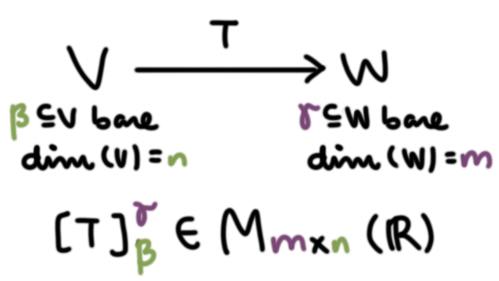
\includegraphics[scale= 1.9]{19} 
\end{marginfigure}
Así, una vez fijadas las bases $\beta$ y $\gamma$, 
\textbf{la transformación lineal $T$ queda completamente determinada
por los $m \times n$ escalares $a_{ji}$, con $1 \leq i \leq n$ y
$1 \leq j \leq m$}. Almacenamos esta información en la siguiente
matriz:

\begin{equation}
	\label{eq: representacion matricial T}
	[T]_{\beta}^{\gamma} = 
	\begin{pmatrix}
	a_{11} & a_{12} & \ldots & a_{1n} \\
	a_{21} & a_{22} & \ldots & a_{2n} \\
	\vdots & \vdots & \ddots & \vdots \\
	a_{m1} & a_{m2} & \ldots & a_{mn} 
	\end{pmatrix}.
\end{equation}
Note que la $i-$ésima columna de $[T]_{\beta}^{\gamma}$
es el vector columna $[T(v_{i})]_{\gamma}$. Entonces,
\begin{itemize}
	\item La matriz $[T]_{\beta}^{\gamma}$ tiene $n$ columnas,
	pues hay una por cada elemento de la base $\beta$ de $V$, y
	\item tiene $m$ filas, pues cada vector columna tiene $m$ 
	entradas, a saber, los coeficientes de las combinaciones
	lineales de las imágenes $T(v_{i})$ respecto a $\gamma$.
\end{itemize}

\begin{figure}[H]
	\sidecaption{
	Este diagrama puede ayudarte a recordar cómo se construye
	la matriz
	$[T]_{\beta}^{\gamma}$
	\label{fig: diagrama representacion matr}
	}
	\centering
	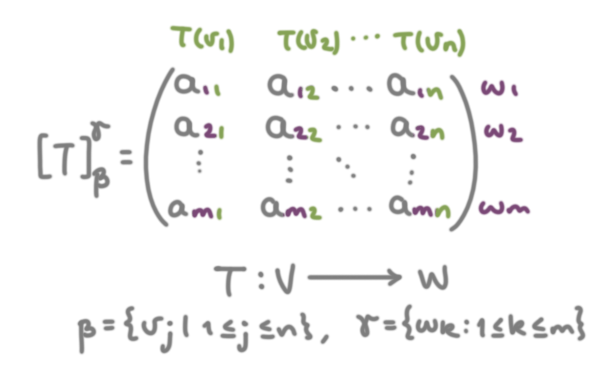
\includegraphics[scale = 2.7]{20} 
\end{figure}	

\section{El isomorfismo $\Phi_{\beta}^{\gamma}$}

Fijadas bases $\beta = \{ v_{j}  | \hspace{0.2cm} 1 \leq j \leq n \}
 \subseteq V$ y $\gamma 
= \{ w_{k}  | \hspace{0.2cm} 1 \leq k \leq n \} 
 \subseteq W$ de dos 
$F-$espacios finito dimensionales, se puede establecer una biyección
entre
\begin{itemize}
	\item el espacio $\mathcal{L}(V, W)$ de transformaciones lineales
	de $V$ en $W$ y 
	\item el espacio de matrices $M_{m \times n}(F)$;
\end{itemize}
vamos a denotar por 
$\Phi_{\beta}^{\gamma}$ a la función que a cada 
transformación lineal de $V$ en $W$ le asigna su representación
matricial respecto a $\beta$ y $\gamma$, i.e.
\[
\Phi_{\beta}^{\gamma} : \mathcal{L}(V, W) \longrightarrow M_{m \times n}(F)
\]
\[
\Phi_{\beta}^{\gamma}(T) = [T]_{\beta}^{\gamma}.
\]

Del teorema fundamental de las bases se sigue fácilmente
el que $\Phi_{\beta}^{\gamma}$ sea biyectiva.

\begin{prop}
La función $\Phi_{\beta}^{\gamma}$ es una biyección.
\end{prop}
\noindent
\textbf{Demostración.}
\begin{itemize}
	\item \textbf{Inyectividad de $\Phi_{\beta}^{\gamma}$}:
	Sean $T, U : V \longrightarrow W$ lineales tales que 
	\[
	[T]_{\beta}^{\gamma} = \Phi_{\beta}^{\gamma}(T)
	= \Phi_{\beta}^{\gamma}(T) = [U]_{\beta}^{\gamma}.
	\]
	El que las matrices $[T]_{\beta}^{\gamma}$ y 
$[U]_{\beta}^{\gamma}$ sean iguales significa que 
\[
\forall v \in \beta : \hspace{0.2cm} T(v) = U(v)
\]
pues la $j-$ésima columna de esta matriz da los coeficientes 
de la combinación lineal en términos de $\gamma$ igual a $T$ evaluada en el
$j-$ésimo vector de la base $\beta$. Así, $T$ y $U$ coinciden en la 
base $\beta$ de $V$, luego, según el corolario 
\ref{cor: del teor fund bases}, coinciden.
	\item \textbf{Suprayectividad de $\Phi_{\beta}^{\gamma}$}:
	sea $A = (a_{ij}) \in M_{m \times n}(F)$. Por el teorema fundamental 
	de las bases, 
	existe una única
transformación lineal tal que 
\[
T(v_{j}) = \sum_{k = 1}^{m} a_{kj} w_{j}, \hspace{0.3cm}
1 \leq j \leq n.
\]
Dicha $T$ es tal que $[T]_{\beta}^{\gamma} = A$.
\end{itemize}

\QEDB
\vspace{0.2cm}


\begin{cor}
Si $T: V \longrightarrow V$ es una transformación lineal
tal que $[T]_{\beta}^{\beta} = Id_{n}$, entonces $T$ es la función
identidad.
\end{cor}






\textbf{Nota:} se pidió a partir de ahora que las bases de los
espacios vectoriales considerados fuesen ordenadas pues,
para la construcción de las representaciones matriciales 
$[T]_{\beta}^{\gamma}$, la $j-$ésima columna corresponde al
$j-$ésimo vector de la base $\beta$, luego, el orden en el que se
enlistan los elementos de $\beta$ importa (es cierto que un cambio
de orden en los elementos de un conjunto no afecta su identidad,
pero el cambiar el orden de las filas o columnas de una matriz la 
altera).

En la siguiente sección desarrollaremos la teoría suficiente
para demostrar que, más que una biyección, $\Phi_{\beta}^{\gamma}$
es un isomorfismo. Esto implica que el espacio
$\mathcal{L}(V, W)$ de transformaciones lineales entre
dos espacios finito dimensionales es 
(salvo isomorfismo) un espacio de matrices. En lo que sigue
seguiremos estudiando y explotando la relación entre dos espacios,
para interpretar las operaciones que realicemos en uno en
términos de operaciones en el otro espacio (pues, para las aplicaciones,
es muchísimo más sencillo trabajar con matrices a lidiar
con transformaciones lineales entre espacios que, a pesar de ser
finito dimensionales, pueden ser complicados).

\section{Operaciones entre transformaciones lineales con sus representaciones matriciales}

\begin{prop}
Sean
$V$ y $W$ dos $F-$espacios vectoriales con $\beta = \{ v_{1}, \ldots , 
v_{n} \} \subseteq V$ y 
$\gamma = \{ w_{1}, \ldots , w_{m}\} \subseteq W$ bases de estos. 
\marginnote{Nota que el lado izquierdo de 
\eqref{eq: suma de matrices transf lin} involucra una suma de funciones,
mientras que el lado derecho es una suma de matrices.}
Para cualesquiera $T, U :V \longrightarrow W$, 
\begin{equation}
	\label{eq: suma de matrices transf lin}
	[T + U]_{\beta}^{\gamma} = [T]_{\beta}^{\gamma} + 
[U]_{\beta}^{\gamma}.
\end{equation}
\end{prop}

\begin{prop}
	\label{prop: calculo de composicion de transf a partir de producto de matr}
Sean $V$, $W$ y $Z$ tres $F-$espacios vectoriales,
con
$\beta = \{ v_{j} : \hspace{0.2cm} 1 \leq j \leq n \} \subseteq V$,
$\gamma = \{ w_{k}: \hspace{0.2cm} 1 \leq k \leq m \} \subseteq W$
y $\delta = \{ z_{i}: \hspace{0.2cm} 1 \leq i \leq r \}$
bases de estos. Si
\marginnote{Nota que el lado izquierdo de 
\eqref{eq: multipl de matrices transf lin} involucra una 
composición de funciones,
mientras que el lado derecho es un producto de matrices.
De hecho, el producto de matrices se definió de tal forma que
la ecuación \eqref{eq: multipl de matrices transf lin} fuese cierta.}
$T: V \longrightarrow W$ y $U: W \longrightarrow Z$ son lineales,
entonces
 \begin{equation}
	\label{eq: multipl de matrices transf lin}
	[U \circ T]_{\beta}^{\delta} = [U]_{\gamma}^{\delta} \cdot  
[T]_{\beta}^{\gamma}.
\end{equation}
\end{prop}
\noindent
\textbf{Demostración.}
Tenemos que $[U]_{\gamma}^{\delta} \in M_{r \times m}(\IR)$
y que $[T]_{\beta}^{\gamma} \in M_{m \times n}(\IR)$, por lo tanto, 
el producto de matrices en 
\eqref{eq: multipl de matrices transf lin} está bien definido.
\begin{center}
$[U]_{\gamma}^{\delta}$ tiene $1 \leq i \leq r$ filas y 
$1 \leq k \leq m$ columnas,
\end{center}
\begin{center}
$[T]_{\beta}^{\gamma}$ tiene $1 \leq k \leq m$ filas y 
$1 \leq j \leq n$ columnas;
\end{center}
entonces,
\begin{center}
$[U \circ T]_{\beta}^{\delta}$ tiene $1 \leq i \leq r$ filas y 
$1 \leq j \leq n$ columnas.
\end{center}

\begin{center}
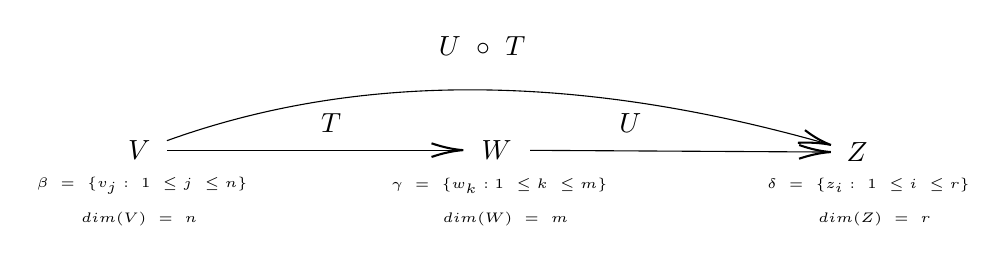
\begin{tikzpicture}[x=0.75pt,y=0.75pt,yscale=-1,xscale=1.4]
%uncomment if require: \path (0,235); %set diagram left start at 0, and has height of 235


% Text Node
\draw (123,131) node    {$V$};
% Text Node
\draw (246,131) node    {$W$};
% Text Node
\draw (370,132) node    {$Z$};
% Text Node
\draw (189,118) node    {$T$};
% Text Node
\draw (292,118) node    {$U$};
% Text Node
\draw (241,81) node    {$U\ \circ \ T$};
% Text Node
\draw (124,148) node  [font=\tiny]  {$\beta \ =\ \{v_{j} :\ 1\ \leq j\ \leq n \}$};
% Text Node
\draw (247,148) node  [font=\tiny]  {$\gamma \ =\ \{w_{k} :1\ \leq k\ \leq m \}$};
% Text Node
\draw (374,148) node  [font=\tiny]  {$\delta \ =\ \{z_{i} :\ 1\ \leq i\ \leq r\}$};
% Text Node
\draw (123,164) node  [font=\tiny]  {$dim( V) \ =\ n$};
% Text Node
\draw (249,164) node  [font=\tiny]  {$dim( W) \ =\ m$};
% Text Node
\draw (376,164) node  [font=\tiny]  {$dim( Z) \ =\ r$};
% Connection
\draw    (132.5,131) -- (232.5,131) ;
\draw [shift={(234.5,131)}, rotate = 180] [color={rgb, 255:red, 0; green, 0; blue, 0 }  ][line width=0.75]    (10.93,-3.29) .. controls (6.95,-1.4) and (3.31,-0.3) .. (0,0) .. controls (3.31,0.3) and (6.95,1.4) .. (10.93,3.29)   ;
% Connection
\draw    (257.5,131.09) -- (359,131.91) ;
\draw [shift={(361,131.93)}, rotate = 180.46] [color={rgb, 255:red, 0; green, 0; blue, 0 }  ][line width=0.75]    (10.93,-3.29) .. controls (6.95,-1.4) and (3.31,-0.3) .. (0,0) .. controls (3.31,0.3) and (6.95,1.4) .. (10.93,3.29)   ;
% Connection
\draw    (132.5,126.45) .. controls (198.12,93.27) and (273.85,93.77) .. (359.7,127.98) ;
\draw [shift={(361,128.49)}, rotate = 201.89] [color={rgb, 255:red, 0; green, 0; blue, 0 }  ][line width=0.75]    (10.93,-3.29) .. controls (6.95,-1.4) and (3.31,-0.3) .. (0,0) .. controls (3.31,0.3) and (6.95,1.4) .. (10.93,3.29)   ;

\end{tikzpicture}
\end{center}


Digamos pues que
\[
[U]_{\gamma}^{\delta} = 
\begin{pmatrix}
a_{11} & a_{12} & \ldots & a_{1m} \\
a_{21} & a_{22} & \ldots & a_{2m} \\
\vdots & \vdots & \ddots & \vdots \\
a_{r1} & a_{r2} & \ldots & a_{rm}
\end{pmatrix},
\hspace{0.2cm}
[T]_{\beta}^{\gamma} = 
\begin{pmatrix}
b_{11} & b_{12} & \ldots & b_{1n} \\
b_{21} & b_{22} & \ldots & b_{2n} \\
\vdots & \vdots & \ddots & \vdots \\
b_{k1} & b_{k2} & \ldots & b_{kn}
\end{pmatrix};
\]
estas dos ecuaciones matriciales equivalen a los siguientes
dos grupos de ecuaciones: 
\[
\forall 1 \leq j \leq n: \hspace{0.3cm}
T(v_{j}) = \sum_{k = 1}^{m} b_{kj} w_{k}
\]
y
\[
\forall 1 \leq k \leq m: \hspace{0.3cm}
U(w_{k}) = \sum_{i= 1}^{r} a_{ik} z_{i}.
\]

Ahora bien, la $j-$ésima columna de $[U \circ T]_{\beta}^{\delta}$
se consigue evaluando a $U \circ T$ en $v_{j}$:
\begin{align*}
(U \circ T)(v_{j}) = & U (T(v_{j})) = 
U\left( \sum_{k=1}^{m} b_{kj} w_{k} \right) \\
= & \sum_{k=1}^{m} b_{kj} U(w_{k}) = 
\sum_{k=1}^{m} b_{kj} \left( \sum_{i=1}^{r} a_{ik} z_{i} \right) \\
= & \sum_{i=1}^{r} \left( \sum_{k=1}^{m} a_{ik} b_{kj} \right) z_{i};
\end{align*}
reconociendo a $\sum_{k=1}^{m} a_{ik} b_{kj}$ como la $ij-$ésima
entrada del producto 
$[U]_{\gamma}^{\delta} \cdot  
[T]_{\beta}^{\gamma}$, terminamos.

\QEDB
\vspace{0.2cm}

\begin{lema}
	\label{lema: Ab como comb lineal de vectores col de A}
Sean $A = (a_{kj})_{\substack{ 1 \leq k \leq m \\ 1 \leq j \leq n }}
\in M_{m \times n} (F)$, $b = (b_{j})_{1 \leq j \leq n} \in M_{n \times 1}(F)$.
Si por $A_{., j}$ denotamos a la $j-$ésima columna de $A$, entonces
\marginnote{Nótese que la ecuación 
\eqref{eq: Ab como comb lineal de vectores col de A}
tiene sentido, pues tanto $Ab$ como los vectores columna de $A$ tienen
dimensión $m \times 1$.}
\begin{equation}
	\label{eq: Ab como comb lineal de vectores col de A}
	Ab = b_{1} A_{., 1} + \ldots + b_{n} A_{., n}, 
\end{equation}
es decir, $Ab$ es una combinación lineal de las columnas de $A$, 
donde los escalares de la combinación lineal son las entradas de $b$.
\end{lema}
\noindent
\textbf{Demostración.}
En efecto, la $k-$ésima entrada tanto de $Ab$ como de 
$\sum_{j = 1}^{n} A_{., j} b_{j}$
es $\sum_{j = 1}^{n}a_{kj}b_{j}$ ($k$ se mantiene fijo y se itera
el índice de columnas $j$ de $A$).

\begin{figure}[H]
\centering\captionsetup{format = hang}
		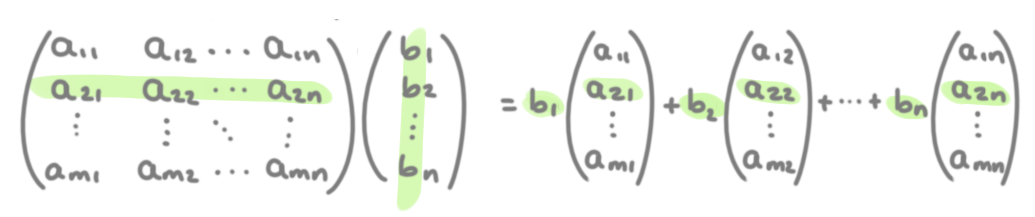
\includegraphics[scale=2.5]{21}
 \end{figure}
\QEDB 
\vspace{0.2cm}

\begin{teo}
	\label{teo: calculando Tx en terminos de representaciones matriciales}
Sean $V$ y $W$ dos $F-$espacios vectoriales finito dimensionales.
Si $\beta \subseteq V$ y $\gamma \subseteq W$ son bases de estos espacios
y $T: V \longrightarrow W$ es una transformación lineal, 
entonces, 
\[
\forall x \in V: \hspace{0.3cm} 
[T(x)]_{\gamma} = [T]_{\beta}^{\gamma} [x]_{\beta}.
\]
\end{teo}
\noindent
\textbf{Demostración.}
En efecto, 
si $\beta \ =\ \{v_{j} :\ 1\ \leq j\ \leq n \}$ y
\[
[x]_{\beta} = \begin{pmatrix}
x_{1} \\
\vdots \\
x_{n}
\end{pmatrix},
\hspace{0.2cm} \textit{ i.e. si }
x = \sum_{j=1}^{n} x_{i}v_{i},
\]
usando el Lema \ref{lema: Ab como comb lineal de vectores col de A},
se sigue de inmediato que 
\begin{align*}
[T]_{\beta}^{\gamma} = & 
x_{1} [T(v_{1})]_{\gamma} + x_{2} [T(v_{2})]_{\gamma} + \cdots + 
x_{n}[T(v_{n})]_{\gamma} \\
= & [x_{1}T(v_{1}) + \cdots + 
x_{n} T(v_{n})]_{\gamma} \\
= & [T(x_{1}v_{1} + \cdots + x_{n}v_{n})] = [T(x)]_{\gamma}.
\end{align*}

\QEDB
\vspace{0.2cm}

\section{Transformaciones lineales de la forma $L_{A}$}
Sea $A \in M_{m \times n} (F)$ una matriz de $m$ filas y 
$n$ columnas con coeficientes en $F$. Definimos a partir de ella
una transformación lineal como sigue:

\begin{equation}
	\label{eq: La}
L_{A} : F^{n} \longrightarrow F^{m}
\end{equation}
\[
L_{A}(x) = Ax,
\]
o sea, $L_{A}$ es la función ``multiplicar a $A$ por la izquierda
de vectores de $F^{n}$''.

Usando esta nueva notación, podemos establecer el teorema
\ref{teo: calculando Tx en terminos de representaciones matriciales} en 
términos del siguiente diagrama de transformaciones lineales:
 
 \marginnote{Este diagrama representa lo explicado en el Teorema
 \ref{teo: calculando Tx en terminos de representaciones matriciales}.}
\begin{center}
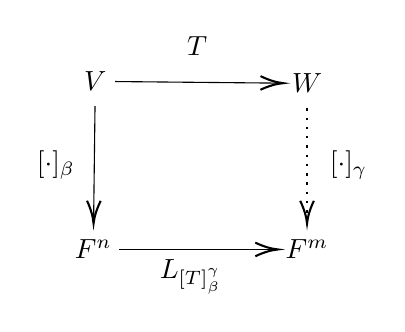
\begin{tikzpicture}[x=0.75pt,y=0.75pt,yscale=-1,xscale=1]
\draw (85,82.14) node    {$V$};
% Text Node
\draw (187,83.14) node    {$W$};
% Text Node
\draw (187,163.14) node    {$F^{m}$};
% Text Node
\draw (134,65.29) node    {$T$};
% Text Node
\draw (66,122.29) node    {$[ \cdot ]_{\beta }$};
% Text Node
\draw (84,163.14) node    {$F^{n}$};
% Text Node
\draw (207,122.29) node    {$[ \cdot ]_{\gamma }$};
% Text Node
\draw (131,176.29) node    {$L_{[T]_{\beta}^{\gamma}}$};
% Connection
\draw    (94.5,82.24) -- (173.5,83.01) ;
\draw [shift={(175.5,83.03)}, rotate = 180.56] [color={rgb, 255:red, 0; green, 0; blue, 0 }  ][line width=0.75]    (10.93,-3.29) .. controls (6.95,-1.4) and (3.31,-0.3) .. (0,0) .. controls (3.31,0.3) and (6.95,1.4) .. (10.93,3.29)   ;
% Connection
\draw  [dash pattern={on 0.84pt off 2.51pt}]  (187,95.14) -- (187,148.64) ;
\draw [shift={(187,150.64)}, rotate = 270] [color={rgb, 255:red, 0; green, 0; blue, 0 }  ][line width=0.75]    (10.93,-3.29) .. controls (6.95,-1.4) and (3.31,-0.3) .. (0,0) .. controls (3.31,0.3) and (6.95,1.4) .. (10.93,3.29)   ;
% Connection
\draw    (96.5,163.14) -- (171,163.14) ;
\draw [shift={(173,163.14)}, rotate = 180] [color={rgb, 255:red, 0; green, 0; blue, 0 }  ][line width=0.75]    (10.93,-3.29) .. controls (6.95,-1.4) and (3.31,-0.3) .. (0,0) .. controls (3.31,0.3) and (6.95,1.4) .. (10.93,3.29)   ;
% Connection
\draw    (84.85,94.14) -- (84.18,148.64) ;
\draw [shift={(84.15,150.64)}, rotate = 270.71] [color={rgb, 255:red, 0; green, 0; blue, 0 }  ][line width=0.75]    (10.93,-3.29) .. controls (6.95,-1.4) and (3.31,-0.3) .. (0,0) .. controls (3.31,0.3) and (6.95,1.4) .. (10.93,3.29)   ;
\end{tikzpicture}
\end{center}
Es decir,

\[
[\cdot]_{\gamma} \circ T = L_{[T]_{\beta}^{\gamma}} \circ [\cdot]_{\beta}.
\]

Nótese que partimos de espacios vectoriales $V$ y $W$ \textit{arbitrarios}
(siendo la única condición impuesta el que ambos sean finito dimensionales),
y que gracias a los isomorfismos $[\cdot]_{\beta}$ podemos 
usar transformaciones del tipo \eqref{eq: La} en lugar
de transformaciones $T: V \longrightarrow W$.

Algunas propiedades fáciles de probar sobre transformaciones
de la forma \eqref{eq: La} se enuncian y se dejan como ejercicio.
\begin{prop}
Si $L_{A}$ es como se definió en \eqref{eq: La}, entonces
\begin{itemize}
	\item $L_{A}$ es lineal
	\item Si $\beta$ y $\gamma$ son las bases canónicas de
	$F^{n}$ y $F^{m}$ respectivamente, entonces $[L_{A}]_{\beta}^{\gamma} = A$.
	\item $L_{A} = L_{B}$ si y sólo si $A = B$.
	\item $L_{A + B} = L_{A} + L_{B}$ y $L_{\lambda A} = \lambda L_{A}$
	para toda $\lambda \in F$.
	\item Si $T: F^{n} \longrightarrow F^{m}$ es una transformación lineal,
	entonces existe una única matriz $C$ de $m \times n$ tal que 
	$T = L_{C}$
	\item Si $E$ es una matriz de $n \times r$, entonces
	$L_{AE} = L_{A} \circ L_{E}$.
\end{itemize} 
\end{prop}

Veremos a continuación que la invertibilidad de 
una transformación lineal
$T$ (i.e. el que sea o no isomorfismo) está 
relacionada a la de cualquiera de sus representaciones matriciales
$[T]_{\beta}^{\gamma}$.

\marginnote{Recuerda que una matriz $A$ es invertible si y sólo si
$A$ es cuadrada y
existe $B$ otra matriz tal que $A B = I_{n} = B A$.}
\begin{teo}
Sea $T: V \longrightarrow W$ una transformación lineal entre dos
$F-$espacios vectoriales finito dimensionales $V$ y $W$.
Si $\beta \subseteq V$ y $\gamma \subseteq W$ son bases cualesquiera
de estos, entonces $T$ es un isomorfismo si y sólo si la matriz
$[T]_{\beta}^{\gamma}$ es invertible.
\end{teo}
\noindent
\textbf{Demostración.}
\begin{itemize}
	\item[$\Rightarrow$)] Supongamos que $T$ es un isomorfismo, es decir,
	que es invertible. Entonces, según la proposición 
	\ref{prop: isomorfo implica misma dimension}, $dim(V) = dim(W)$.
	Sean $\beta = \{ v_{j}  | \hspace{0.2cm} 1 \leq j \leq n \}$ y
	$\gamma \{ w_{j}  | \hspace{0.2cm} 1 \leq j \leq n \}$ bases de $V$
	y $W$, y sea $T^{-1}: W \longrightarrow V$ la inversa de $T$ - que, 
	recuerde, también es una transformación lineal. Entonces, 
	según la proposición
	\ref{prop: calculo de composicion de transf a partir de producto de matr},
	\[
	I_{n} = [I_{V}]_{\beta}^{\beta} = [T^{-1} \circ T]_{\beta}^{\beta}
	= [T^{-1}]_{\gamma}^{\beta} [T]_{\beta}^{\gamma}
	\]
	y, análogamente,
	\[
	I_{n} = [T]_{\beta}^{\gamma} [T^{-1}]_{\gamma}^{\beta}.
	\]
	Así, $[T]_{\beta}^{\gamma}$ es invertible y, de hecho,
	\marginnote{La ecuación \eqref{eq: inversa de repr matr de T} es 
	importante en sí misma.}
	\begin{equation}
		\label{eq: inversa de repr matr de T}
		([T]_{\beta}^{\gamma})^{-1} = [T^{-1}]_{\gamma}^{\beta}.
	\end{equation}
	
	\item[$\Leftarrow$)] Sea $B \in M_{n \times n}(F)$ tal que
	\[
	[T]_{\beta}^{\gamma}B = I_{n} = B [T]_{\beta}^{\gamma}.
	\]
	Entonces, si $U: W \longrightarrow V$ es la única transformación lineal
	tal que $[U]_{\gamma}^{\beta} = B$, 
	\[
	[T \circ U]_{\gamma}^{\gamma} = [T]_{\beta}^{\gamma} [U]_{\gamma}^{\beta}
	= I_{n}.
	\]
	Esto implica que $T \circ U$ es la identidad en $W$. De forma
	análoga se prueba que $U \circ T$ es la identidad en $V$. Así,
	$T$ es invertible, luego, un isomorfismo.
\end{itemize}

\QEDB
\vspace{0.2cm}

\begin{prop}
Fijadas $\beta \subseteq V$ y $\gamma \subseteq W$ bases de los
$F-$espacios vectoriales finito dimensionales $V$ y $W$, 
la función 
\[
\Phi_{\beta}^{\gamma} : \mathcal{L}(V, W) \longrightarrow M_{m \times n}(F)
\]
\[
\Phi_{\beta}^{\gamma}(T) = [T]_{\beta}^{\gamma}.
\]
es un isomorfismo.
\end{prop}
\noindent
\textbf{Demostración.}
Ya vimos en proposciones anteriores la linealidad de 
$\Phi_{\beta}^{\gamma}$. 
\begin{itemize}
	\item Inyectividad: si $T: V \longrightarrow W$ es tal que
	$[T]_{\beta}^{\gamma}$ es la matriz cero, entonces $T$
	evaluada en cualquier vector de la base $\beta$ es cero, luego,
	$T$ debe ser la transformación lineal cero. Así,
	$Ker(\Phi_{\beta}^{\gamma}) = \{ 0 \}$.
	
	\item Suprayectividad: se estableció en la proposición 
	\ref{prop: suprayectividad de phi beta gamma}.
\end{itemize}

\QEDB
\vspace{0.2cm}

\begin{cor}
Si $dim(V) = n$ y $dim(W) = m$, entonces el espacio 
$\mathcal{L}(V, W)$ de transformaciones lineales de $V$ a $W$
es finito dimensional, de hecho,
$dim(\mathcal{L}(V, W)) = mn$.
\end{cor}

\section{Ejemplos}
Sea
\[
\mathcal{U}_{2}(\IR) = \left\{
\begin{pmatrix}
a & b \\
0 & c
\end{pmatrix}: \hspace{0.2cm}
a, b, c \in \IR
\right\} \leq M_{2 \times 2}
\]
el subespacio de matrices triangulares superiores de $2 \times 2$.
No es difícil convencerse de que este es un $\IR-$ espacio vectorial
de dimensión $3$, de hecho,
\[
\delta = \left\{
\begin{pmatrix}
1 & 0 \\
0 & 0
\end{pmatrix}, 
\begin{pmatrix}
0 & 1 \\
0 & 0
\end{pmatrix}, 
\begin{pmatrix}
0 & 0 \\
0 & 1
\end{pmatrix}
\right\}
\]
es una base para $\mathcal{U}_{2}(\IR)$.
Sean las transformaciones lineales
$S : \mathcal{U}_{2}(\IR) \longrightarrow \IR^{3}$,
$T: \mathbb{U}_{2}(\IR) \longrightarrow U_{2}(\IR)$
definidas como

\[
T \begin{pmatrix}
a & b \\
0 & c
\end{pmatrix} = 
\begin{pmatrix}
a & b \\
0 & a
\end{pmatrix} ,
\]
\[
U
\begin{pmatrix}
a & b \\
0 & c
\end{pmatrix} = 
(a, b, c)
\]

\section{Cambio de sistema coordenado}

\begin{signquote}{Mac Lane, 1954}
    The proper treatment of calculus for functions of 
several variables requires vector ideas; the budding statistician and
the coming physicist need them; modern 
analysis is unthinkable without the notion of linear
dependence and all that flows from it. Throughout these
courses the infusion of a geometrical point of view is of paramount 
importance. A vector is geometrical; it is an element of a vector space,
defined by suitable axioms - whether the scalars be real numbers or
elements of a general field. A vector is not an n-tuple of numbers
until a coordinate system has been chosen. Any teacher and any
text book which starts with the idea that vectors are
n-tuples is committing a crime for which the proper punishment is ridicule.
The n-tuple idea is not ``easier'', it is harder; it is not clearer, it is
more misleading. 
\end{signquote}


Ya ha quedado claro el uso de una base en un $F-$espacio 
vectorial $V$; estas actuan como un
\textbf{sistema de coordenadas}, pues, como se estableción
en el teorema \ref{teo: equiv de base}
(resultado usado una y otra vez en el desarrollo
de la teoría anterior), si $\beta$ es base de $V$,
dado $x \in V$ \textit{cualquiera}, existen
\begin{itemize}
	\item \textbf{únicos} $v_{1}, \ldots, v_{n}$ de elementos 
	de $\beta$, y
	\item \textbf{únicos} escalares $a_{1}, \ldots, a_{n}$ escalares
	tales que
\end{itemize}
\[
x = \sum_{j = 1}^{n} a_{i} x_{i}.
\]
Recuerde que es por eso que, en el caso en el que $V$ es finito dimensional
(i.e. $\beta$ es finita), usamos esto para construir el isomorfismo
$[\cdot]_{\beta}$ entre $V$ y $F^{n}$ (justo asociándole a $x$ su única
colección de escalares $a_{1}, \ldots, a_{n}$). Note que esta representación
\textbf{depende de la base $\beta$}, es decir, si $\gamma \subseteq V$
es una base de $V$ distinta a $\beta$, entonces los isomorfismos
$[\cdot]_{\beta}$
y $[\cdot]_{\gamma}$ son distintos entre sí. Un caso particular de esta
situación es el realizar un cambio de coordenadas en el plano
(el espacio vectorial en esta situación es, por supuesto, $\IR^{2}$).

En este caso, ``fijar el plano/sistema coordenado'' y
``fijar la base'' significan lo mismo.
\TODO{Discusión del pizarrón. Fijar sistema de referencia, y usar nuevas
bases en ese sitema.}
\begin{ejem}
Mostremos cómo en ocasiones es conveniente cambiar de sistema de coordenadas.
En $\IR^{2}$, considere a la base canónica $\beta = \{ 
e_{1} = (1, 0), e_{2} = (0, 1) \}$.
Todo punto del espacio $(x, y)$ se expresa de forma única como combinación
lineal de elementos de $\beta$;
\[
(x, y) = x(1, 0) + y(0,1).
\]
Esta representación es muy sencilla - por eso resulta ventajoso en muchas
ocasiones trabajar con la base canónica de $\IR^{2}$. Considere al lugar 
geométrico $\mathcal{E} \subseteq \IR^{2}$ de puntos del plano que 
consta de los puntos que satisfacen la siguiente relación:
\begin{equation}
	\label{eq: elipse 1}
	w = (x, y) \in \mathcal{E} \hspace{0.2cm} \textit{ si y sólo si }
	\hspace{0.2cm}
	2x^{2} - 4xy + 5 y^{2} = 1.
\end{equation}
Puesto que en la ecuación para definir $\mathcal{E}$ están
involucrados cuadrados de las variables, parece que este lugar
geométrico es una cónica, sin embargo,
el término mixto $-4xy$ dificulta su identificación. Cambiemos 
de sistema coordenado; considérese a la base

\[
\beta' = \left\{
u = \left( \frac{\sqrt{5}}{5}, -\frac{2 \sqrt{5}}{5} \right),
v = \left( \frac{2\sqrt{5}}{5}, \frac{\sqrt{5}}{5} \right)
\right\}.
\]
Si $w = (x, y) \in \IR^{2}$, entonces
\begin{align*}
w = (x, y) = & x e_{1} + y e_{2} \\
= & x'u + y' v \\
= &  x' \left( \frac{\sqrt{5}}{5}, -\frac{2 \sqrt{5}}{5} \right) 
+ y' \left( \frac{2\sqrt{5}}{5}, \frac{\sqrt{5}}{5} \right) \\
= &x' \left( \frac{\sqrt{5}}{5} e_{1} -
\frac{2\sqrt{5}}{5} e_{2} \right)
+ y' \left( \frac{2\sqrt{5}}{5}e_{1} + 
\frac{\sqrt{5}}{5} e_{2} \right) \\
= & \left( \frac{\sqrt{5}}{5} x' + \frac{2\sqrt{5}}{5} y' \right)e_{1} + 
\left( -\frac{2\sqrt{5}}{5} x' + \frac{\sqrt{5}}{5}y' \right) e_{2}.
\end{align*}

\marginnote{A esta situación se le conoce en geometría analítica como
``eliminación del término mixto''.}

De la igualdad de los coeficientes al representar vectores respecto a una
base se deduce que 
\begin{equation}
	\label{eq: relacion x x' cambio base ejemplo}
	x = \frac{\sqrt{5}}{5} x' + \frac{2\sqrt{5}}{5} y', 
	\hspace{0.2cm}
	y =  -\frac{2\sqrt{5}}{5} x' + \frac{\sqrt{5}}{5}y'.
\end{equation}
Si usamos ahora el sistema coordenado $\beta'$, debemos sustituir 
los cambios \eqref{eq: relacion x x' cambio base ejemplo}
en la condición de definición \eqref{eq: elipse 1}. Haciendo esto, 
llegamos a que 
\begin{equation}
	\label{eq: elipse 2}
	w = x'u + y'v \in \mathcal{E} 
	\hspace{0.2cm} \textit{ si y sólo si }
	\hspace{0.2cm}
	6(x')^{2} + (y')^{2} = 1.
\end{equation}
Ahora sí reconocemos al lugar geométrico como una elipse, pero 
\textbf{no} respecto al sistema coordenado $\beta$, sino respecto 
a $\beta'$.
\begin{marginfigure}
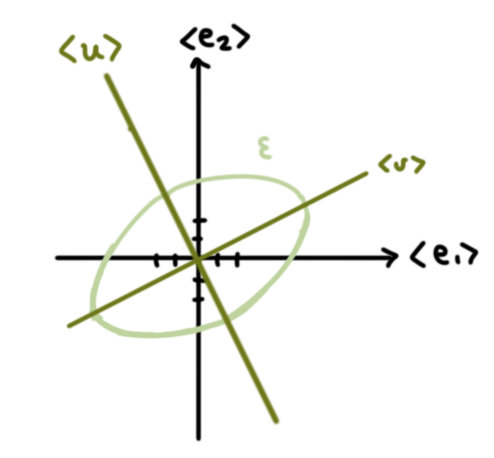
\includegraphics[scale= 2.3]{22}
\end{marginfigure}

Al dibujar el nuevo sistema coordenado en el plano (i.e. a las 
rectas $\langle \{ u \} \rangle$ y $\langle \{ v \} \rangle$, que son 
subespacios uno dimensionales de $\IR^{2}$), notamos que este se 
obtiene rotando el sistema original $\beta$.

Observa que la relación 
\eqref{eq: relacion x x' cambio base ejemplo}
(que nos permitió pasar de una base a otra) puede representarse
en forma matricial como 
\[
\begin{pmatrix}
x \\ y
\end{pmatrix} = 
\begin{pmatrix}
\frac{\sqrt{5}}{5} & \frac{2\sqrt{5}}{5} \\
-\frac{2\sqrt{5}}{5} & \frac{\sqrt{5}}{5}
\end{pmatrix}
\begin{pmatrix}
x' \\ y'
\end{pmatrix};
\]
nota que 
\[
[w]_{\beta} = \begin{pmatrix}
x \\ y
\end{pmatrix},
\hspace{0.2cm}
[Id]_{\beta'}^{\beta} = 
\begin{pmatrix}
\frac{\sqrt{5}}{5} & \frac{2\sqrt{5}}{5} \\
-\frac{2\sqrt{5}}{5} & \frac{\sqrt{5}}{5}
\end{pmatrix},
\hspace{0.2cm}
[w]_{\beta'} = \begin{pmatrix}
x' \\ y'
\end{pmatrix}.
\]
\end{ejem}

Usando el que la transformación lineal identidad es el neutro de
la composición y que multiplicación de matrices es la operación 
correspondiente a composición de funciones, se establece fácilmente
cómo hacer cambios de base.

\begin{teo}
Sean $\beta$, $\beta'$ dos bases de un $F-$espacio vectorial finito 
dimensional $V$. Sea $Q = [Id_{V}]_{\beta'}^{\beta}$.
\begin{itemize}
	\item La matriz $Q$ es invertible.
	\item Para toda $v \in V$,
	\begin{equation}
		\label{eq: v beta igual a id por v beta prima}
		[v]_{\beta} = Q [v]_{\beta'}.
	\end{equation}
\end{itemize}
\end{teo}
\marginnote{La ecuación \eqref{eq: v beta igual a id por v beta prima}
nos explica cómo obtener las coordenadas de un vector $v$
en términos de $\beta$ cuando se tienen sus coordenadas en 
términos de $\beta'$.}
\noindent
\textbf{Demostración.}
Claro que $Q$ es invertible, pues la transformación identidad
$Id_{V}$ es un isomorfismo (c.f. \TODO{cita}).
Además, según 
el Teorema \ref{teo: calculando Tx en terminos de representaciones matriciales},
\[
[v]_{\beta} = [Id_{V}(v)]_{\beta} = [Id]_{\beta'}^{\beta}[v]_{\beta'}.
\]
\QEDB
\vspace{0.2cm}

\begin{defi}
Si $\beta$ y $\beta'$ son dos bases de un $F-$espacio vectorial
finito dimensional $V$, a la matriz $[Id]_{\beta'}^{\beta}$
se le conoce como \textbf{matriz de cambio de base} de 
$\beta'$ a $\beta$.
\end{defi}

\TODO{Poner ejemplo numérico.}

Sean $V$ y $W$ dos $F-$espacios vectoriales, y considere dos pares de bases
\[
\beta \subseteq V, \gamma \subseteq W;
\hspace{0.4cm}
\beta' \subseteq V, \gamma' \subseteq W
\]
de estos.
Dada una transformación lineal $T: V \longrightarrow W$,
según el Teorema 
\ref{teo: calculando Tx en terminos de representaciones matriciales},
tenemos los siguientes dos cuadrados conmutativos;
\TODO{cambia flecha punteada}
\begin{center}
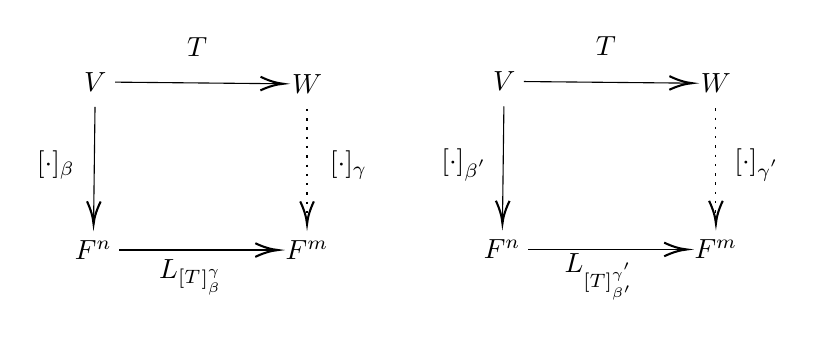
\begin{tikzpicture}[x=0.75pt,y=0.75pt,yscale=-1,xscale=1]
%uncomment if require: \path (0,235); %set diagram left start at 0, and has height of 235


% Text Node
\draw (85,82.14) node    {$V$};
% Text Node
\draw (187,83.14) node    {$W$};
% Text Node
\draw (187,163.14) node    {$F^{m}$};
% Text Node
\draw (134,65.29) node    {$T$};
% Text Node
\draw (66,122.29) node    {$[ \cdot ]_{\beta }$};
% Text Node
\draw (84,163.14) node    {$F^{n}$};
% Text Node
\draw (207,122.29) node    {$[ \cdot ]_{\gamma }$};
% Text Node
\draw (131,176.29) node    {$L_{[ T}{}_{]_{\beta }^{\gamma }}$};
% Text Node
\draw (282,81.86) node    {$V$};
% Text Node
\draw (384,82.86) node    {$W$};
% Text Node
\draw (384,162.86) node    {$F^{m}$};
% Text Node
\draw (331,65) node    {$T$};
% Text Node
\draw (263,122) node    {$[ \cdot ]_{\beta ^{'}}$};
% Text Node
\draw (281,162.86) node    {$F^{n}$};
% Text Node
\draw (404,122) node    {$[ \cdot ]_{\gamma ^{'}}$};
% Text Node
\draw (328,176) node    {$L_{[T]_{\beta'}^{\gamma^{'}}}$};
% Connection
\draw    (94.5,82.24) -- (173.5,83.01) ;
\draw [shift={(175.5,83.03)}, rotate = 180.56] [color={rgb, 255:red, 0; green, 0; blue, 0 }  ][line width=0.75]    (10.93,-3.29) .. controls (6.95,-1.4) and (3.31,-0.3) .. (0,0) .. controls (3.31,0.3) and (6.95,1.4) .. (10.93,3.29)   ;
% Connection
\draw  [dash pattern={on 0.84pt off 2.51pt}]  (187,95.14) -- (187,148.64) ;
\draw [shift={(187,150.64)}, rotate = 270] [color={rgb, 255:red, 0; green, 0; blue, 0 }  ][line width=0.75]    (10.93,-3.29) .. controls (6.95,-1.4) and (3.31,-0.3) .. (0,0) .. controls (3.31,0.3) and (6.95,1.4) .. (10.93,3.29)   ;
% Connection
\draw    (96.5,163.14) -- (171,163.14) ;
\draw [shift={(173,163.14)}, rotate = 180] [color={rgb, 255:red, 0; green, 0; blue, 0 }  ][line width=0.75]    (10.93,-3.29) .. controls (6.95,-1.4) and (3.31,-0.3) .. (0,0) .. controls (3.31,0.3) and (6.95,1.4) .. (10.93,3.29)   ;
% Connection
\draw    (84.85,94.14) -- (84.18,148.64) ;
\draw [shift={(84.15,150.64)}, rotate = 270.71] [color={rgb, 255:red, 0; green, 0; blue, 0 }  ][line width=0.75]    (10.93,-3.29) .. controls (6.95,-1.4) and (3.31,-0.3) .. (0,0) .. controls (3.31,0.3) and (6.95,1.4) .. (10.93,3.29)   ;
% Connection
\draw    (291.5,81.95) -- (370.5,82.72) ;
\draw [shift={(372.5,82.74)}, rotate = 180.56] [color={rgb, 255:red, 0; green, 0; blue, 0 }  ][line width=0.75]    (10.93,-3.29) .. controls (6.95,-1.4) and (3.31,-0.3) .. (0,0) .. controls (3.31,0.3) and (6.95,1.4) .. (10.93,3.29)   ;
% Connection
\draw  [dash pattern={on 0.84pt off 2.51pt}]  (384,94.86) -- (384,148.36) ;
\draw [shift={(384,150.36)}, rotate = 270] [color={rgb, 255:red, 0; green, 0; blue, 0 }  ][line width=0.75]    (10.93,-3.29) .. controls (6.95,-1.4) and (3.31,-0.3) .. (0,0) .. controls (3.31,0.3) and (6.95,1.4) .. (10.93,3.29)   ;
% Connection
\draw    (293.5,162.86) -- (368,162.86) ;
\draw [shift={(370,162.86)}, rotate = 180] [color={rgb, 255:red, 0; green, 0; blue, 0 }  ][line width=0.75]    (10.93,-3.29) .. controls (6.95,-1.4) and (3.31,-0.3) .. (0,0) .. controls (3.31,0.3) and (6.95,1.4) .. (10.93,3.29)   ;
% Connection
\draw    (281.85,93.86) -- (281.18,148.36) ;
\draw [shift={(281.15,150.36)}, rotate = 270.71] [color={rgb, 255:red, 0; green, 0; blue, 0 }  ][line width=0.75]    (10.93,-3.29) .. controls (6.95,-1.4) and (3.31,-0.3) .. (0,0) .. controls (3.31,0.3) and (6.95,1.4) .. (10.93,3.29)   ;

\end{tikzpicture}
\end{center}
Ambos diagramas hacen referencia a $T$ (su objetivo de hecho es 
decir cómo
evaluar a $T$ en vectores de $V$ en términos de multiplicaciones
de matrices). ¿Qué relación hay entre estos? En otras palabras,
¿Cómo conociendo la representación matricial 
$[T]_{\beta}^{\gamma}$ encontramos a $[T]_{\beta'}^{\gamma'}$?
\begin{center}
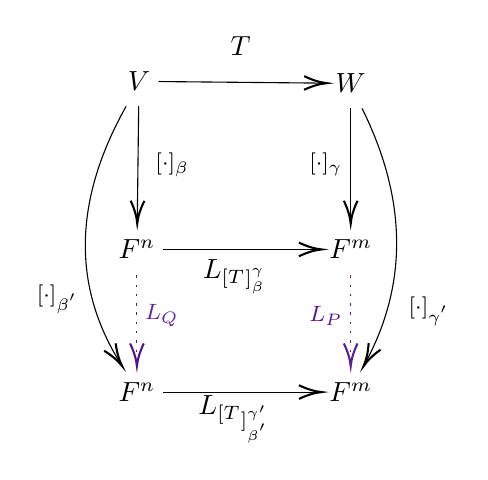
\begin{tikzpicture}[x=0.75pt,y=0.75pt,yscale=-1,xscale=1]
%uncomment if require: \path (0,235); %set diagram left start at 0, and has height of 235


% Text Node
\draw (87,27.14) node    {$V$};
% Text Node
\draw (189,28.14) node    {$W$};
% Text Node
\draw (189,108.14) node    {$F^{m}$};
% Text Node
\draw (136,10.29) node    {$T$};
% Text Node
\draw (103,67.29) node  [font=\footnotesize]  {$[ \cdot ]_{\beta }$};
% Text Node
\draw (86,108.14) node  [color={rgb, 255:red, 0; green, 0; blue, 0 }  ,opacity=1 ]  {$F^{n}$};
% Text Node
\draw (177,67.29) node  [font=\footnotesize]  {$[ \cdot ]_{\gamma }$};
% Text Node
\draw (133,121.29) node    {$L_{[ T}{}_{]_{\beta }^{\gamma }}$};
% Text Node
\draw (189,176.86) node    {$F^{m}$};
% Text Node
\draw (86,176.86) node    {$F^{n}$};
% Text Node
\draw (133,190) node    {$L_{[ T}{}_{]_{\beta ^{'}}^{\gamma '}}$};
% Text Node
\draw (48,132) node  [font=\footnotesize]  {$[ \cdot ]_{\beta ^{'}}$};
% Text Node
\draw (227,138) node  [font=\footnotesize]  {$[ \cdot ]_{\gamma ^{'}}$};
% Text Node
\draw (98,140.14) node  [font=\footnotesize,color={rgb, 255:red, 100; green, 35; blue, 158 }  ,opacity=1 ]  {$L_{Q}$};
% Text Node
\draw (177,140.14) node  [font=\footnotesize,color={rgb, 255:red, 90; green, 15; blue, 151 }  ,opacity=1 ]  {$L_{P}$};
% Connection
\draw    (96.5,27.24) -- (175.5,28.01) ;
\draw [shift={(177.5,28.03)}, rotate = 180.56] [color={rgb, 255:red, 0; green, 0; blue, 0 }  ][line width=0.75]    (10.93,-3.29) .. controls (6.95,-1.4) and (3.31,-0.3) .. (0,0) .. controls (3.31,0.3) and (6.95,1.4) .. (10.93,3.29)   ;
% Connection
\draw    (189,40.14) -- (189,93.64) ;
\draw [shift={(189,95.64)}, rotate = 270] [color={rgb, 255:red, 0; green, 0; blue, 0 }  ][line width=0.75]    (10.93,-3.29) .. controls (6.95,-1.4) and (3.31,-0.3) .. (0,0) .. controls (3.31,0.3) and (6.95,1.4) .. (10.93,3.29)   ;
% Connection
\draw    (98.5,108.14) -- (173,108.14) ;
\draw [shift={(175,108.14)}, rotate = 180] [color={rgb, 255:red, 0; green, 0; blue, 0 }  ][line width=0.75]    (10.93,-3.29) .. controls (6.95,-1.4) and (3.31,-0.3) .. (0,0) .. controls (3.31,0.3) and (6.95,1.4) .. (10.93,3.29)   ;
% Connection
\draw    (86.85,39.14) -- (86.18,93.64) ;
\draw [shift={(86.15,95.64)}, rotate = 270.71] [color={rgb, 255:red, 0; green, 0; blue, 0 }  ][line width=0.75]    (10.93,-3.29) .. controls (6.95,-1.4) and (3.31,-0.3) .. (0,0) .. controls (3.31,0.3) and (6.95,1.4) .. (10.93,3.29)   ;
% Connection
\draw    (98.5,176.86) -- (173,176.86) ;
\draw [shift={(175,176.86)}, rotate = 180] [color={rgb, 255:red, 0; green, 0; blue, 0 }  ][line width=0.75]    (10.93,-3.29) .. controls (6.95,-1.4) and (3.31,-0.3) .. (0,0) .. controls (3.31,0.3) and (6.95,1.4) .. (10.93,3.29)   ;
% Connection
\draw    (80.81,39.14) .. controls (55.48,84.3) and (54.61,125.66) .. (78.18,163.22) ;
\draw [shift={(78.9,164.36)}, rotate = 237.29] [color={rgb, 255:red, 0; green, 0; blue, 0 }  ][line width=0.75]    (10.93,-3.29) .. controls (6.95,-1.4) and (3.31,-0.3) .. (0,0) .. controls (3.31,0.3) and (6.95,1.4) .. (10.93,3.29)   ;
% Connection
\draw    (194.45,40.14) .. controls (216.1,83.77) and (216.67,124.59) .. (196.15,162.62) ;
\draw [shift={(195.2,164.36)}, rotate = 299.15] [color={rgb, 255:red, 0; green, 0; blue, 0 }  ][line width=0.75]    (10.93,-3.29) .. controls (6.95,-1.4) and (3.31,-0.3) .. (0,0) .. controls (3.31,0.3) and (6.95,1.4) .. (10.93,3.29)   ;
% Connection
\draw [color={rgb, 255:red, 82; green, 19; blue, 138 }  ,draw opacity=1 ] [dash pattern={on 0.84pt off 2.51pt}]  (86,120.64) -- (86,162.36) ;
\draw [shift={(86,164.36)}, rotate = 270] [color={rgb, 255:red, 82; green, 19; blue, 138 }  ,draw opacity=1 ][line width=0.75]    (10.93,-3.29) .. controls (6.95,-1.4) and (3.31,-0.3) .. (0,0) .. controls (3.31,0.3) and (6.95,1.4) .. (10.93,3.29)   ;
% Connection
\draw [color={rgb, 255:red, 91; green, 29; blue, 147 }  ,draw opacity=1 ] [dash pattern={on 0.84pt off 2.51pt}]  (189,120.64) -- (189,162.36) ;
\draw [shift={(189,164.36)}, rotate = 270] [color={rgb, 255:red, 91; green, 29; blue, 147 }  ,draw opacity=1 ][line width=0.75]    (10.93,-3.29) .. controls (6.95,-1.4) and (3.31,-0.3) .. (0,0) .. controls (3.31,0.3) and (6.95,1.4) .. (10.93,3.29)   ;

\end{tikzpicture}
\end{center}
Podemos usar matrices de cambio de base para pasar fácilmente de una
representación matricial a la otra. En efecto, 
si 
\[
P = [Id_{W}]_{\gamma}^{\gamma'}, \hspace{0.2cm}
Q = [Id_{V}]_{\beta}^{\beta'}, 
\]
entonces,
para toda $v \in V$,
$$P[T]_{\beta}^{\gamma} [v]_{\beta} = ([Id_{W}]_{\gamma}^{\gamma'}
	[T]_{\beta}^{\gamma})[v_{\beta}] = [Id_{W} \circ T]_{\beta}^{\gamma'}
	[v]_{\beta} = [T]_{\beta}^{\gamma'}[v]_{\beta} = [T(v)]_{\gamma},$$
y también
$$
[T]_{\beta'}^{\gamma'} Q [v]_{\beta} = ([T]_{\beta'}^{\gamma'}
[Id_{V}]_{\beta}^{\beta'})[v]_{\beta} = [T \circ Id_{V}]_{\beta}^{\gamma'}
[v]_{\beta} = [T]_{\beta}^{\gamma'}[v]_{\beta} = [T(v)]_{\gamma}.
$$
De esto se deduce que 
\begin{equation}
	\label{eq: P T beta gama = T beta' gamma' Q}
	P[T]_{\beta}^{\gamma} = [T]_{\beta'}^{\gamma'} Q.
\end{equation}
\marginnote{En efecto, toma a $[v]_{\beta}$ como un vector de la base 
canónica de $F^{n}$ para probar que las correspondientes columnas de 
las matrices en \eqref{eq: P T beta gama = T beta' gamma' Q} en
efecto coinciden entre sí.}
Puesto que $P$ es invertible, podemos despejar a $[T]_{\beta}^{\gamma}$
de \eqref{eq: P T beta gama = T beta' gamma' Q}.
Hemos demostrado así el siguiente 
\begin{teo}
	\label{teo: cambio de bases repr matr}
Sean $V$ y $W$ dos $F-$espacios vectoriales finito dimensionales,
$T: V \longrightarrow W$ una transformación lineal entre ellos.
Si $\beta, \beta' \subseteq V$ y $\gamma, \gamma' \subseteq W$ son 
bases para estos espacios, 
\begin{itemize}
	\item $P = [Id_{W}]_{\gamma}^{\gamma'}$ es la matriz que transforma
	las coordenadas de $\gamma$ en $\gamma'$, y 
	\item $Q = [Id_{V}]_{\beta}^{\beta'}$ es la matriz que transforma
	las coordenadas de $\beta$ en $\beta'$,
\end{itemize}
entonces,
\begin{equation}
	\label{eq: T beta gama = P inv T beta' gamma' Q}
	[T]_{\beta}^{\gamma} = P^{-1} [T]_{\beta'}^{\gamma'} Q.
\end{equation}
\end{teo}

\begin{obs}
Si $V$ es un $F-$espacio vectorial finito dimensional y 
$\beta, \beta' \subseteq V$ son bases de $V$, entonces
\begin{equation}
	\label{eq: inversa de id beta a beta' es con bases en otro orden}
	([Id_{V}]_{\beta}^{\beta'})^{-1} = [Id_{V}]_{\beta'}^{\beta}.
\end{equation}
\end{obs}

\TODO{Ejemplo numérico con observaciones.}

Vale la pena escribir el Teorema 
\ref{teo: cambio de bases repr matr} para el caso particular 
en el que el espacio de dominio coincide con el de codominio.

\begin{cor}
	\label{cor: T de V en V cambio de base}
Si $V$ es un $F-$espacio vectorial finito dimensional y 
$\beta, \beta' \subseteq V$ son bases de $V$, entonces
\begin{equation}
	\label{eq: T de V en V dos bases}
	[T]_{\beta}^{\beta} = Q^{-1} [T]_{\beta'}^{\beta'} Q,
\end{equation}
donde $Q= [Id_{V}]_{\beta}^{\beta'}$.
\end{cor}

\subsection{Matrices similares}
\TODO{Sigue discusión y salta a 
p. 239 Friedb.}

\begin{defi}
Sean $A, B \in M_{n \times n}(F)$. Decimos que las matrices $A$ y $B$
son \textbf{similares} si existe $Q \in M_{n \times n}(F)$ invertible tal que
\[
A = Q^{-1}B Q.
\]
\end{defi}
En términos de esta definición, el Corolario 
\ref{cor: T de V en V cambio de base} se resume como sigue:
\begin{center}
\textit{Las representaciones matriciales de una transformación lineal
$T: V \longrightarrow V$ respecto a una misma base son todas similares entre
sí.}
\end{center}
No es difícil demostrar que la relación ``ser similar con''
es de equivalencia:
\noindent
\hlgray{Ejercicio:} Demuestra que la relación en el conjunto
de las matrices cuadradas $n \times n$ dada por
\[
\forall A, B \in M_{n \times n}(F): \hspace{0.2cm}
A \sim B \hspace{0.2cm} \Leftrightarrow
\exists Q \in M_{n \times n}(F) \textit{ invertible tal que }
A = Q^{-1}B Q
\]
es de equivalencia, es decir, que 
\begin{itemize}
	\item es reflexiva: $\forall A \in M_{n \times n}(F): A \sim A$,
	\item simétrica: $\forall A, B \in M_{n \times n}(F): A \sim B
	\Rightarrow B \sim A$, y
	\item transitiva: $\forall A, B, C \in M_{n \times n}(F):
	A \sim B \wedge B \sim C \Rightarrow A \sim C$.
\end{itemize}

Como toda relación de equivalencia, esta induce una partición
en el conjunto $M_{n \times n}(F)$. Sea $V$ un $F-$espacio vectorial
con $dim(V) = n$ (por ejemplo, $V = F^{n}$).

\begin{center}
\begin{figure}[H]
\centering
		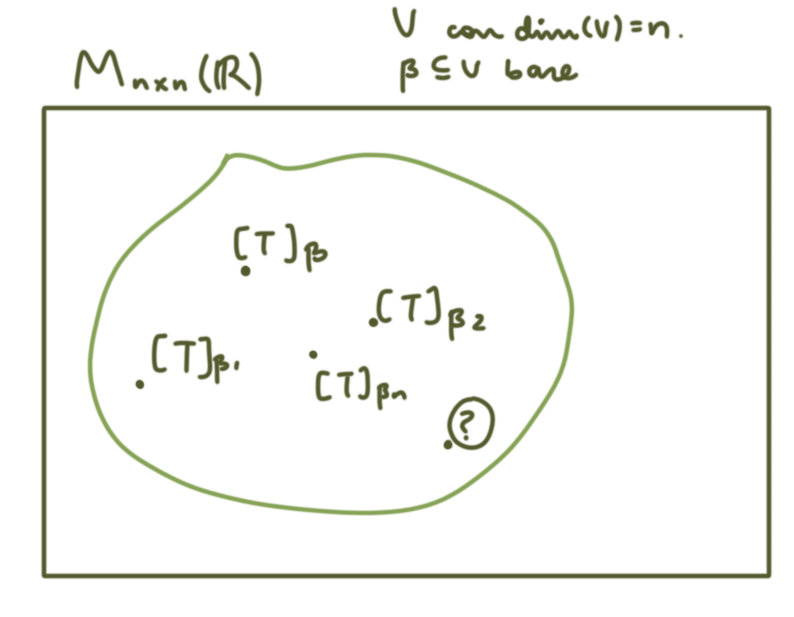
\includegraphics[scale=3]{23}
 \end{figure}
\end{center}
